\documentclass[12pt, a4paper]{article}
% Some fancy symbols
\usepackage{textcomp}
\usepackage{stmaryrd}
\usepackage{cancel}

% Some fancy symbols
\usepackage{textcomp}
\usepackage{stmaryrd}


\usepackage{array}

% Math packages
\usepackage{amsmath,amsthm,amssymb, amsfonts, mathrsfs, dsfont, mathtools}
% \usepackage{mathtext}

\usepackage[bb=boondox]{mathalfa}
\usepackage{bm}

% To conrol figures:
\usepackage{subfig}
\usepackage{adjustbox}
\usepackage{placeins}
\usepackage{rotating}



\usepackage{lipsum}
\usepackage{psvectorian} % Insanely fancy text separators!


% Refs:
\usepackage{url}
\usepackage[backref]{hyperref}

% Fancier tables and lists
\usepackage{booktabs}
\usepackage{enumitem}
% Don't indent paragraphs, leave some space between them
\usepackage{parskip}
% Hide page number when page is empty
\usepackage{emptypage}


\usepackage{multicol}
\usepackage{xcolor}

\usepackage[normalem]{ulem}

% For beautiful code listings:
% \usepackage{minted}
\usepackage{listings}

\usepackage{csquotes} % For citations
\usepackage[framemethod=tikz]{mdframed} % For further information see: http://marcodaniel.github.io/mdframed/

% Plots
\usepackage{pgfplots} 
\pgfplotsset{width=10cm,compat=1.9} 

% Fonts
\usepackage{unicode-math}
% \setmathfont{TeX Gyre Termes Math}

\usepackage{fontspec}
\usepackage{polyglossia}

% Named references to sections in document:
\usepackage{nameref}


% \setmainfont{Times New Roman}
\setdefaultlanguage{russian}

\newfontfamily\cyrillicfont{Kurale}
\setmainfont[Ligatures=TeX]{Kurale}
\setmonofont{Fira Code}

% Common number sets
\newcommand{\sN}{{\mathbb{N}}}
\newcommand{\sZ}{{\mathbb{Z}}}
\newcommand{\sZp}{{\mathbb{Z}^{+}}}
\newcommand{\sQ}{{\mathbb{Q}}}
\newcommand{\sR}{{\mathbb{R}}}
\newcommand{\sRp}{{\mathbb{R^{+}}}}
\newcommand{\sC}{{\mathbb{C}}}
\newcommand{\sB}{{\mathbb{B}}}

% Math operators

\makeatletter
\newcommand\RedeclareMathOperator{%
  \@ifstar{\def\rmo@s{m}\rmo@redeclare}{\def\rmo@s{o}\rmo@redeclare}%
}
% this is taken from \renew@command
\newcommand\rmo@redeclare[2]{%
  \begingroup \escapechar\m@ne\xdef\@gtempa{{\string#1}}\endgroup
  \expandafter\@ifundefined\@gtempa
     {\@latex@error{\noexpand#1undefined}\@ehc}%
     \relax
  \expandafter\rmo@declmathop\rmo@s{#1}{#2}}
% This is just \@declmathop without \@ifdefinable
\newcommand\rmo@declmathop[3]{%
  \DeclareRobustCommand{#2}{\qopname\newmcodes@#1{#3}}%
}
\@onlypreamble\RedeclareMathOperator
\makeatother


% Correction:
\definecolor{correct_color}{HTML}{009900}
\newcommand\correction[2]{\ensuremath{\:}{\color{red}{#1}}\ensuremath{\to }{\color{correct_color}{#2}}\ensuremath{\:}}
\newcommand\inGreen[1]{{\color{correct_color}{#1}}}

% Roman numbers && fancy symbs:
\newcommand{\RNumb}[1]{{\uppercase\expandafter{\romannumeral #1\relax}}}
\newcommand\textbb[1]{{$\mathbb{#1}$}}



% MD framed environments:
\mdfsetup{skipabove=1em,skipbelow=0em}

% \mdfdefinestyle{definition}{%
%     linewidth=2pt,%
%     frametitlebackgroundcolor=white,
%     % innertopmargin=\topskip,
% }

\theoremstyle{definition}
\newmdtheoremenv[nobreak=true]{definition}{Определение}
\newmdtheoremenv[nobreak=true]{theorem}{Теорема}
\newmdtheoremenv[nobreak=true]{lemma}{Лемма}
\newmdtheoremenv[nobreak=true]{problem}{Задача}
\newmdtheoremenv[nobreak=true]{property}{Свойство}
\newmdtheoremenv[nobreak=true]{statement}{Утверждение}
\newmdtheoremenv[nobreak=true]{corollary}{Следствие}
\newtheorem*{note}{Замечание}
\newtheorem*{example}{Пример}

% To mark logical parts
\newcommand{\existence}{{\circled{$\exists$}}}
\newcommand{\uniqueness}{{\circled{$\hspace{0.5px}!$}}}
\newcommand{\rightimp}{{\circled{$\Rightarrow$}}}
\newcommand{\leftimp}{{\circled{$\Leftarrow$}}}


% Useful symbols:
\renewcommand{\qed}{\ensuremath{\blacksquare}}
\renewcommand{\vec}[1]{\overrightarrow{#1}}
\newcommand{\eqdef}{\overset{\mathrm{def}}{=\joinrel=}}
\newcommand{\isdef}{\overset{\mathrm{def}}{\Longleftrightarrow}}
\newcommand{\inductdots}{\ensuremath{\overset{induction}{\cdots}}}

% Matrix's determinant
\newenvironment{detmatrix}
{
  \left|\begin{matrix}
}{
  \end{matrix}\right|
}

\newenvironment{complex}
{
  \left[\begin{gathered}
}{
  \end{gathered}\right.
}


\newcommand{\nl}{$~$\\}

\newcommand{\tit}{\maketitle\newpage}
\newcommand{\tittoc}{\tit\tableofcontents\newpage}


\newcommand{\vova}{  
    Латыпов Владимир (конспектор)\\
    {\small \texttt{t.me/donRumata03}, \texttt{github.com/donRumata03}, \texttt{donrumata03@gmail.com}}
}


\usepackage{tikz}
\newcommand{\circled}[1]{\tikz[baseline=(char.base)]{
            \node[shape=circle,draw,inner sep=2pt] (char) {#1};}}

\newcommand{\contradiction}{\circled{!!!}}

% Make especially big math:

\makeatletter
\newcommand{\biggg}{\bBigg@\thr@@}
\newcommand{\Biggg}{\bBigg@{4.5}}
\def\bigggl{\mathopen\biggg}
\def\bigggm{\mathrel\biggg}
\def\bigggr{\mathclose\biggg}
\def\Bigggl{\mathopen\Biggg}
\def\Bigggm{\mathrel\Biggg}
\def\Bigggr{\mathclose\Biggg}
\makeatother


% Texts dividers:

\newcommand{\ornamentleft}{%
    \psvectorian[width=2em]{2}%
}
\newcommand{\ornamentright}{%
    \psvectorian[width=2em,mirror]{2}%
}
\newcommand{\ornamentbreak}{%
    \begin{center}
    \ornamentleft\quad\ornamentright
    \end{center}%
}
\newcommand{\ornamentheader}[1]{%
    \begin{center}
    \ornamentleft
    \quad{\large\emph{#1}}\quad % style as desired
    \ornamentright
    \end{center}%
}


% Math operators

\DeclareMathOperator{\sgn}{sgn}
\DeclareMathOperator{\id}{id}
\DeclareMathOperator{\rg}{rg}
\DeclareMathOperator{\determinant}{det}

\DeclareMathOperator{\Aut}{Aut}

\DeclareMathOperator{\Sim}{Sim}
\DeclareMathOperator{\Alt}{Alt}



\DeclareMathOperator{\Int}{Int}
\DeclareMathOperator{\Cl}{Cl}
\DeclareMathOperator{\Ext}{Ext}
\DeclareMathOperator{\Fr}{Fr}


\RedeclareMathOperator{\Re}{Re}
\RedeclareMathOperator{\Im}{Im}


\DeclareMathOperator{\Img}{Im}
\DeclareMathOperator{\Ker}{Ker}
\DeclareMathOperator{\Lin}{Lin}
\DeclareMathOperator{\Span}{span}

\DeclareMathOperator{\tr}{tr}
\DeclareMathOperator{\conj}{conj}
\DeclareMathOperator{\diag}{diag}

\expandafter\let\expandafter\originald\csname\encodingdefault\string\d\endcsname
\DeclareRobustCommand*\d
  {\ifmmode\mathop{}\!\mathrm{d}\else\expandafter\originald\fi}

\newcommand\restr[2]{{% we make the whole thing an ordinary symbol
  \left.\kern-\nulldelimiterspace % automatically resize the bar with \right
  #1 % the function
  \vphantom{\big|} % pretend it's a little taller at normal size
  \right|_{#2} % this is the delimiter
  }}

\newcommand{\splitdoc}{\noindent\makebox[\linewidth]{\rule{\paperwidth}{0.4pt}}}

% \newcommand{\hm}[1]{#1\nobreak\discretionary{}{\hbox{\ensuremath{#1}}}{}}


% \usepackage{geometry}
% \geometry{
%     a4paper,
%     left=30mm,
%     right=30mm,
%     top=30mm,
%     bottom=20mm
% }


\author{Латыпов Владимир Витальевич, \\ ИТМО КТ M3138, \Huge{\textit{\textbf{вариант 12}}}}
\title{Типовик по линейной алгебре модуль 1: Задание 7 «Каноническая форма кривых второго порядка»}

\begin{document}
    \tittoc

    \section{Формулировка условия}

    \begin{statement}
        Условие таково: 
        
        Выполнив последовательно преобразования координат: поворот, а
        затем параллельный перенос координатных осей, преобразовать к
        каноническому виду уравнение кривой второго порядка и построить ее в
        канонической и исходной системе координат, а также найти параметры
        кривой.

        12. $7\sqrt{5} x^2 + \sqrt{5}y^2 + 8\sqrt{5}xy + 72x + 36y + 27\sqrt{5} = 0$
    \end{statement}

    \section{Решение}


    \subsection{Поворот системы координат}
    
    Для начала найдём такой поворот, чтобы член $x'y'$ исчез.
    \begin{equation}
        \begin{cases}
            x = cos(\alpha) x' - sin(\alpha) y' \\
            y = sin(\alpha) x' + cos(\alpha) y'
        \end{cases}
    \end{equation}

    Тогда уравение превращается в:
    \begin{multline}
        7\sqrt{5} (cos(\alpha) x' - sin(\alpha) y')^2 \\
        + \sqrt{5}(sin(\alpha) x' + cos(\alpha) y')^2 \\
        + 8\sqrt{5}(cos(\alpha) x' - sin(\alpha) y')(sin(\alpha) x' + cos(\alpha) y') \\
        + 72 (cos(\alpha) x' - sin(\alpha) y') \\
        + 36 (sin(\alpha) x' + cos(\alpha) y') \\
        + 27\sqrt{5}
    \end{multline}

    После expansion получается:
    \begin{multline}
        7 \sqrt{5} x'^2\cos^2\left(α\right) \\
        + \sqrt{5}x'^2\sin^2\left(α\right) \\
        + 8\sqrt{5}x'^2\cos \left(α\right)\sin \left(α\right) \\
        + 8\sqrt{5}x'y'\cos^2\left(α\right) \\
        - 8\sqrt{5}x'y'\sin ^2\left(α\right) \\
        - 12\sqrt{5}x'y'\sin \left(α\right)\cos \left(α\right) \\
        + 72x'\cos \left(α\right) \\
        + 36x'\sin \left(α\right) \\
        + 7\sqrt{5}y'^2\sin ^2\left(α\right) \\
        + \sqrt{5}y'^2\cos ^2\left(α\right) \\
        - 8\sqrt{5}y'^2\sin \left(α\right)\cos \left(α\right) \\
        - 72y'\sin \left(α\right) \\
        + 36y'\cos \left(α\right) \\
        + 27\sqrt{5}
    \end{multline}

    Выделяем члены с $x' y'$:
    \begin{equation}
        + 8\sqrt{5}x'y'\cos^2\left(α\right) \\
        - 8\sqrt{5}x'y'\sin ^2(α) \\
        - 12\sqrt{5}x'y'\sin (α) \cos(α)
    \end{equation}

    Тогда коэффициент перед $x'y'$ будет:
    \begin{multline}
        7\sqrt{5} \left( -2 cos(\alpha) sin(\alpha) \right) + 8\sqrt{5} \left( cos^2(\alpha) - sin^2(\alpha) \right) + \sqrt{5} \left( 2 cos(\alpha) sin(\alpha) \right) = \\
        \sqrt{5} ( cos(\alpha) sin(\alpha) (7 \cdot -2 + 2) + 8 cos^2(\alpha) - 8 sin^2(\alpha) )
    \end{multline}

    Этот коэффициент должен быть равен нулю. Тогда:
    \begin{gather}
        -12 cos(\alpha) sin(\alpha) + 8cos^2(\alpha) - 8sin^2(\alpha) = 0 \\
        -12tg(\alpha) + 8 - 8tg^2(\alpha) = 0 \\
        4\xi^2 + 6\xi - 4 = 0 \\
        \xi_{1, 2} = \{ -2, \frac{1}{2} \}
    \end{gather}

    Для любого $\alpha$ с одним из этих тангенсов (таких $\alpha$ всего 4) исчезнет перекрёсный член в новой системе координат.

    Возьмём, например, $tg(\alpha) = \frac{1}{2}$ и $\alpha \in (0, \frac{\pi}{2})$.
    Будет $\alpha = arctg\left( \frac{1}{2} \right)$
    Тогда $sin, cos > 0$
    \begin{gather}
        sin(\alpha) = \frac{tg(\alpha)}{\sqrt{1 + tg^2(\alpha)}} = \frac{1}{2} \frac{1}{\sqrt{\frac{5}{4}}} = \frac{1}{\sqrt{5}} = \frac{\sqrt{5}}{5} \\
        cos(\alpha) = \frac{1}{\sqrt{1 + tg^2(\alpha)}} = \frac{1}{\sqrt{\frac{5}{4}}} = \frac{2}{\sqrt{5}} = \frac{2\sqrt{5}}{5}
    \end{gather}

    Тогда старые координаты так выражаются через новые:
    \begin{equation}
        \begin{cases}
            x = \frac{2\sqrt{5}}{5} x' - \frac{\sqrt{5}}{5} y' \\
            y = \frac{\sqrt{5}}{5} x' + \frac{2\sqrt{5}}{5} y'
        \end{cases}
    \end{equation}

    И новая система коодинат будет выглядеть вот так относительно старой:

    \begin{figure}[h!]
        \centering
        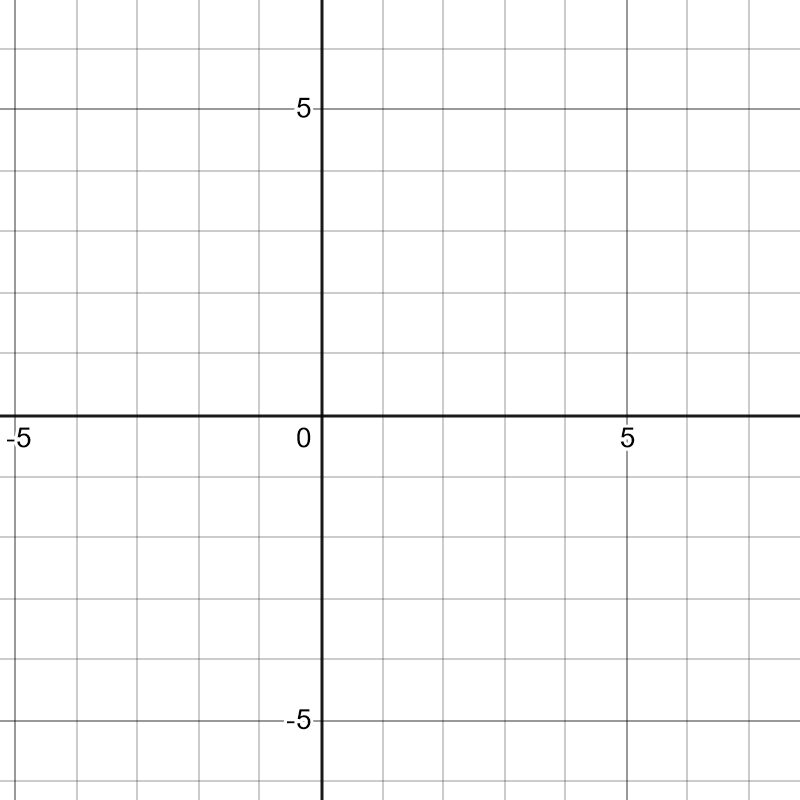
\includegraphics[width=\textwidth]{resources/1.7_grid_x'.png}
        \caption{Система координат $(X', Y')$ относительно исходной}
        \label{fig:grid_1}
    \end{figure}
    \FloatBarrier
    

    Тогда перепишем уравнение в новой системе коодинат:
    \begin{multline}
        7\sqrt{5} \left(\frac{2\sqrt{5}}{5} x' - \frac{\sqrt{5}}{5} y'\right)^2 + \\
        \sqrt{5} \left(\frac{\sqrt{5}}{5} x' + \frac{2\sqrt{5}}{5} y'\right)^2 + \\
        8\sqrt{5} \left(\frac{2\sqrt{5}}{5} x' - \frac{\sqrt{5}}{5} y'\right)\left(\frac{\sqrt{5}}{5} x' + \frac{2\sqrt{5}}{5} y'\right) + \\
        72 \left(\frac{2\sqrt{5}}{5} x' - \frac{\sqrt{5}}{5} y'\right) + \\
        36 \left(\frac{\sqrt{5}}{5} x' + \frac{2\sqrt{5}}{5} y' \right) + \\
        27\sqrt{5} \\
        = 0
    \end{multline}

    \begin{multline}
        \frac{28 x'^2}{\sqrt{5}} - \frac{28 x' y'}{\sqrt{5}} + \frac{7 y'^2}{\sqrt{5}} + \\
        \frac{x'^2}{\sqrt{5}} + \frac{4 x' y'}{\sqrt{5}} + \frac{4 y'^2}{\sqrt{5}} + \\
        \frac{16 x'^2}{\sqrt{5}} + \frac{24 x' y'}{\sqrt{5}} - \frac{16 y'^2}{\sqrt{5}} + \\
        \frac{144 x'}{\sqrt{5}} - \frac{72 y'}{\sqrt{5}} + \\
        \frac{36 x'}{\sqrt{5}} + \frac{72 y'}{\sqrt{5}} + \\
        27\sqrt{5} \\
        = 0
    \end{multline}

    Получили:
    \begin{equation}
        9x'^2 + 36'x - y'^2 + 27 = 0
    \end{equation}

    \subsection{Параллельный перенос}

    Выделим полные квадраты:
    \begin{equation}
        9x'^2 + 36x' - y'^2 + 27 = 9(x'^2 + 4x' + 4) - y'^2 - 9 = 9(x' + 2)^2 - y'^2 - 9 = 0
    \end{equation}
    
    Назовём, получив выражение координат системы $(X', Y')$ через $(X'', Y'')$ и наоборот:
    \begin{equation}
        \begin{cases}
            x'' = x' + 2 \\
            y'' = y'
        \end{cases} \\
        \begin{cases}
            x' = x'' - 2 \\
            y' = y''
        \end{cases}
    \end{equation}
    
    \begin{figure}[h!]
        \centering
        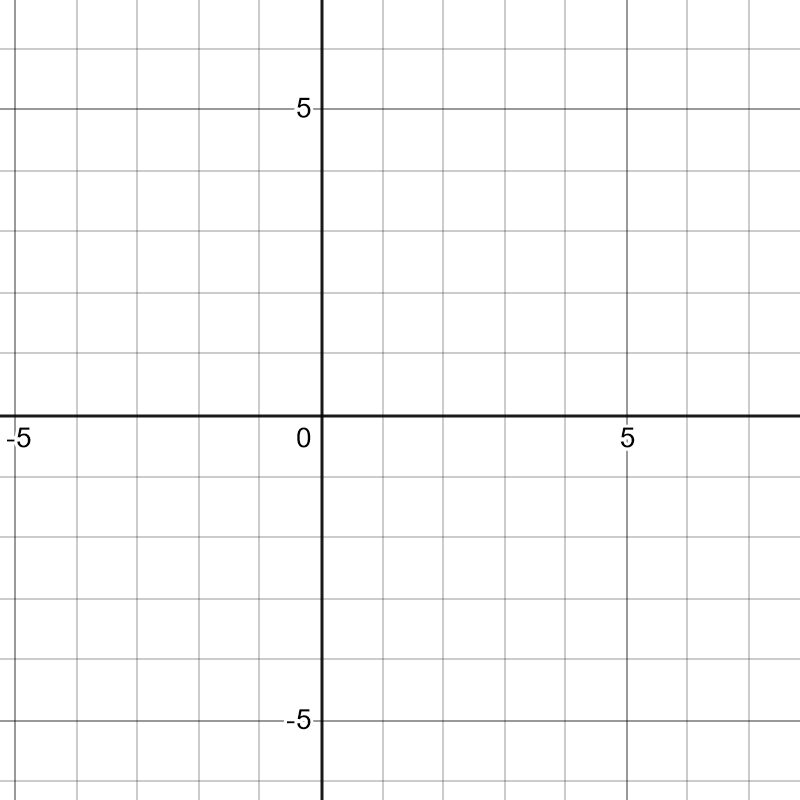
\includegraphics[width=\textwidth]{resources/1.7_grid_x'.png}
        \caption{Система координат $(O'', X'', Y'')$ относительно СК $(O', X', Y')$}
        \label{fig:grid_2}
    \end{figure}
    \FloatBarrier

    \section{Малювание в системе координат два штриха}

    Тогда уравнение в системе координат «два штриха» будет таким:
    
    \begin{equation}
        9x''^2 - y'^2 = 9
    \end{equation}

    \begin{equation}
        \frac{x''^2}{1^2} - \frac{y'^2}{3^2} = 1
    \end{equation}

    То есть это гипербола, главная полуось: $a = 1$, 
    мнимая полуось: $b = 3$,
    $c = \sqrt{a^2 + b^2} = \sqrt{1 + 9} = \sqrt{10}$.
    Ещё параметры гиперболы:

    \begin{gather}
        \varepsilon = \frac{c}{a} = \frac{\sqrt{10}}{1} = \sqrt{10} \\
        F_l, F_r = (\mp c; 0) = (\mp \sqrt{10}; 0) \\
        V_l, V_r = (\mp a; 0)
        D_l, D_r: x'' = \mp \frac{a}{\varepsilon} = \mp \frac{1}{\sqrt{10}} = \mp \frac{\sqrt{10}}{10}
    \end{gather}

    И выглядеть она будет:
    
    \begin{figure}[h!]
        \centering
        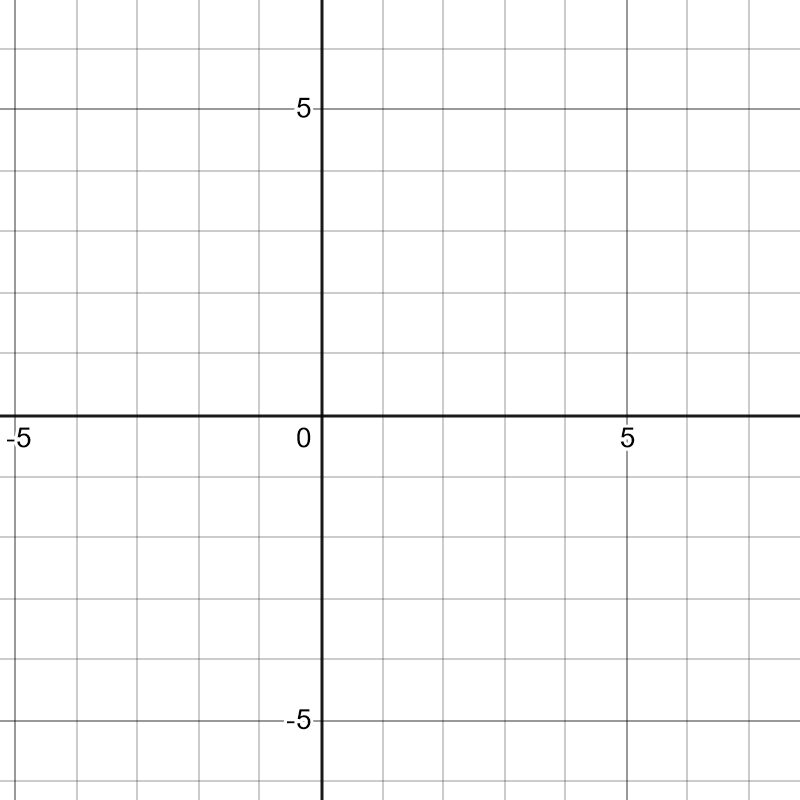
\includegraphics[width=\textwidth]{resources/1.7_grid_x'.png}
        \caption{Гипербола в системе координат $(O'', X'', Y'')$}
        \label{fig:grid_3}
    \end{figure}
    \FloatBarrier


    \section{Итоговое преобразование координат}

    Таким образом, координаты для системы «один штрих» будут выражаться как:
    \begin{equation}
        \begin{cases}
            x' = x'' - 2 \\
            y' = y''
        \end{cases}
    \end{equation}
    (То есть сдвиг влево относительно двух штрихов на 2)

    А для изначальной СК:
    \begin{gather}
        \begin{cases}
            x = cos(\alpha) x' - sin(\alpha) y' = cos(\alpha) (x'' - 2) - sin(\alpha) y'' = \frac{2 \sqrt{5}}{5} (x'' - 2) - \frac{\sqrt{5}}{5} y'' \\
            y = sin(\alpha) x' + cos(\alpha) y' = \frac{\sqrt{5}}{5} (x'' - 2) + \frac{2 \sqrt{5}}{5} y''
        \end{cases} \\
        \begin{cases}
            x = \frac{2 \sqrt{5}}{5} x'' - \frac{\sqrt{5}}{5} y'' - \frac{4 \sqrt{5}}{5} \\
            y = \frac{\sqrt{5}}{5} x'' + \frac{2 \sqrt{5}}{5} y'' - \frac{2 \sqrt{5}}{5}
        \end{cases}
    \end{gather}

    Пользуясь этим, мы можем найти координаты ключевых характеристических фигур нашей гиперболы.

    Во-первых — $O''$ в исходной СК: $\left( -\frac{4 \sqrt{5}}{5}; -\frac{2 \sqrt{5}}{5} \right) \approx (-1.8; -0.9)$.

    Далее — в расход идут вершины и фокусы. В новой системе:
    
    \begin{equation}
        V_1, V_2 =
            \left(
                \frac{2 \sqrt{5}}{5} \cdot (\mp 1) - \frac{4 \sqrt{5}}{5};
                \frac{\sqrt{5}}{5} \cdot (\mp 1) - \frac{2 \sqrt{5}}{5} 
            \right)
    \end{equation}

    \begin{equation}
        V_1, V_2 =
            \left(
                \frac{2 \sqrt{5}}{5} \cdot (\mp 1) - \frac{4 \sqrt{5}}{5};
                \frac{\sqrt{5}}{5} \cdot (\mp 1) - \frac{2 \sqrt{5}}{5} 
            \right)
    \end{equation}

    \begin{gather}
        V_1 \approx
            \left(
                -2.7; -1.3 
            \right) \\
        V_2 \approx
        \left(
            -0.9; -0.5
        \right)
    \end{gather}
     

    \begin{equation}
        F_1, F_2 =
            \left(
                \frac{2 \sqrt{5}}{5} \cdot (\mp \sqrt{10}) - \frac{4 \sqrt{5}}{5};
                \frac{\sqrt{5}}{5} \cdot (\mp \sqrt{10}) - \frac{2 \sqrt{5}}{5} 
            \right)
    \end{equation}

    \begin{gather}
        F_l \approx \left(
                -4.6; \,
                -2.3
            \right) \\
        F_r \approx \left(
            1.; \,
            .5
        \right)
    \end{gather}

    Выразим наоборот — новые координаты через старые.

    \begin{gather}
        \begin{cases}
            x = \frac{2 \sqrt{5}}{5} x'' - \frac{\sqrt{5}}{5} y'' - \frac{4 \sqrt{5}}{5} \\
            y = \frac{\sqrt{5}}{5} x'' + \frac{2 \sqrt{5}}{5} y'' - \frac{2 \sqrt{5}}{5}
        \end{cases} \\
        \begin{cases}
            x = \frac{2 \sqrt{5}}{5} x'' - \frac{\sqrt{5}}{5} y'' - \frac{4 \sqrt{5}}{5} \\
            2y = \frac{2\sqrt{5}}{5} x'' + \frac{4 \sqrt{5}}{5} y'' - \frac{4 \sqrt{5}}{5}
        \end{cases} \\
        \begin{cases}
            x - 2y = (- \frac{\sqrt{5}}{5} - \frac{4 \sqrt{5}}{5} ) y'' = -\frac{5\sqrt{5}}{5} y'' = -\sqrt{5} y'' \\
            2y = \frac{2\sqrt{5}}{5} x'' + \frac{4 \sqrt{5}}{5} y'' - \frac{4 \sqrt{5}}{5}
        \end{cases} \\
        \begin{cases}
            y'' = \frac{2y - x}{\sqrt{5}} = \frac{2 \sqrt{5}}{5} y - \frac{\sqrt{5}}{5} x \\
            x = \frac{2 \sqrt{5}}{5} x'' - \frac{\sqrt{5}}{5} (\frac{2 \sqrt{5}}{5} y - \frac{\sqrt{5}}{5} x) - \frac{4 \sqrt{5}}{5}
        \end{cases} \\
        \frac{2 \sqrt{5}}{5} x'' = x + \frac{\sqrt{5}}{5} \left(\frac{2 \sqrt{5}}{5} y - \frac{\sqrt{5}}{5} x \right) + \frac{4 \sqrt{5}}{5} \\
        \frac{2 \sqrt{5}}{5} x'' = x + \frac{2}{5} y - \frac{1}{5} x + \frac{4 \sqrt{5}}{5} = \frac{4}{5} x + \frac{2}{5} y + \frac{4 \sqrt{5}}{5} \\
        x'' = \frac{\sqrt{5}}{2} \left( \frac{4}{5} x + \frac{2}{5} y + \frac{4 \sqrt{5}}{5} \right) = \frac{2 \sqrt{5}}{5} x + \frac{\sqrt{5}}{5} y + 2 \\
        \begin{cases}
            x'' = \frac{2 \sqrt{5}}{10} x + \frac{\sqrt{5}}{5} y + 2 \\
            y'' = - \frac{\sqrt{5}}{5} x + \frac{2 \sqrt{5}}{5} y
        \end{cases}
    \end{gather}


    Теперь тяжёлая артилерия: оси координат.

    \begin{multline}
        O''Y'': x'' \equiv 0 \\
        \Longleftrightarrow \frac{2 \sqrt{5}}{5} x + \frac{\sqrt{5}}{5} y + 2 = 0 \\
        \Longleftrightarrow \frac{\sqrt{5}}{5} y = -2 -\frac{2 \sqrt{5}}{5} x \\
        \Longleftrightarrow y = -2\sqrt{5} -\frac{2 \sqrt{5} \times \sqrt{5} }{5} x = -2\sqrt{5} - 2x
    \end{multline}

    \begin{multline}
        O''X'': y'' \equiv 0 \\
        \Longleftrightarrow - \frac{\sqrt{5}}{5} x + \frac{2 \sqrt{5}}{5} y = 0 \\
        \Longleftrightarrow \frac{2 \sqrt{5}}{5} y = \frac{\sqrt{5}}{5} x \\
        \Longleftrightarrow y = \frac{\sqrt{5}}{5} \times \frac{\sqrt{5}}{2} x = \frac{1}{2} x
    \end{multline}


    И, наконец, директриссы:
    
    \begin{gather}
        D_l: x'' = -\frac{\sqrt{10}}{10} \\
        \frac{2 \sqrt{5}}{5} x + \frac{\sqrt{5}}{5} y + 2 = -\frac{\sqrt{10}}{10} \\
        y = -2 x - 2 \sqrt{5} - \frac{\sqrt{2}}{2}
    \end{gather}
    
    \begin{gather}
        D_r: x'' = +\frac{\sqrt{10}}{10} \\
        \frac{2 \sqrt{5}}{5} x + \frac{\sqrt{5}}{5} y + 2 = +\frac{\sqrt{10}}{10} \\
        y = -2 x - 2 \sqrt{5} + \frac{\sqrt{2}}{2}
    \end{gather}

    \section{Итоговая иллюстрация}
    
    Теперь мы можем изобразить гиперболу в исходой системе координат.
    \begin{figure}[h!]
        \centering
        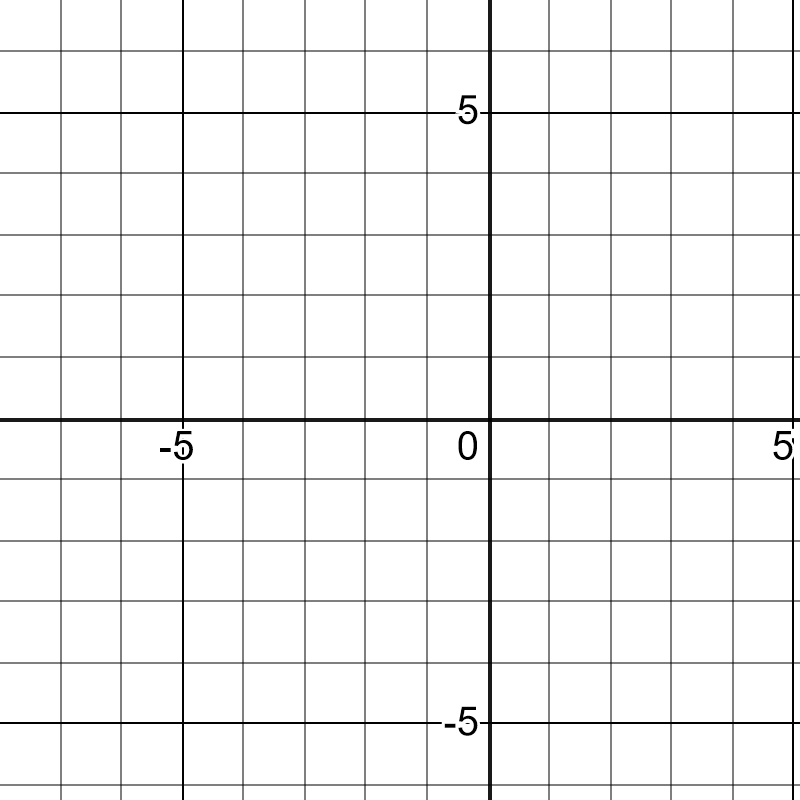
\includegraphics[width=\textwidth]{resources/1.7_grid_left.png}
        \caption{Гипербола в системе координат $(O, X, Y)$}
        \label{fig:grid_4}
    \end{figure}
    \FloatBarrier 
    


\end{document}
